\documentclass[10pt,oneside,a4paper]{article}

\usepackage[]{babel}
\usepackage[IL2]{fontenc}
\usepackage[utf8]{inputenc}
\usepackage{graphicx}
\usepackage{url}
\usepackage{hyperref}
\usepackage{cite}
\usepackage{lipsum}  % Пакет для автогенерации текста, используется для демонстрации объема статьи

\pagestyle{headings}

\title{Challenges in Semantic Search: Understanding User Intent and Context\thanks{Semester Project in Methods of Engineering Work, Academic Year 2022/23}}

\author{Aliaksei Zimnitski \\[2pt]
{\small \texttt{xzimnitski@stuba.sk}}\\
Coauthor: MSc. Mirwais Ahmadzai \\[2pt]
{\small \texttt{mirwais.ahmadzai@stuba.sk}}\\
{\small Slovenská technická univerzita v Bratislave}\\
{\small Fakulta informatiky a informačných technológií}\\
}

\date{\small \today}

\begin{document}

\maketitle

\begin{abstract}
Semantic search is a vital technology in the field of information retrieval. It plays a pivotal role in enhancing search accuracy by focusing on understanding user intent and context. This article delves into the multifaceted challenges faced by semantic search systems, offering insights into the intricacies of ambiguity resolution and the need to adapt to dynamic language. It underscores the importance of leveraging natural language processing and artificial intelligence to address these challenges effectively. By comprehending these complexities, we can unlock the full potential of semantic search in information retrieval.
\end{abstract}


\section{Introduction}
Semantic search has revolutionized information retrieval, offering the promise of more accurate and context-aware search results. However, it is not without its challenges. This paper delves into the intricacies of semantic search and the hurdles it encounters when trying to understand user intent and context.

The advent of semantic search has brought about a paradigm shift in the way we seek and access information. Unlike traditional keyword-based searches, semantic search aims to understand the meaning behind the queries, making it a cornerstone of modern information retrieval. It goes beyond surface-level keyword matching and focuses on deciphering the intricacies of human language, emphasizing user intent and context.

\section{Resolving User Intent Ambiguity}
One of the primary challenges in semantic search is the ambiguity of user intentions. Consider a simple query like "Apple." It could refer to the technology company, the fruit, or even a record label. Semantic search engines must decipher the relevant context to provide accurate results.

To tackle this issue, semantic search systems employ a variety of techniques, including natural language processing, entity recognition, and context analysis. These methods help disambiguate user queries and retrieve relevant results. However, the challenge persists, as language is nuanced and context-dependent.

User intent ambiguity is further compounded by the evolution of language and the emergence of new terms and concepts. For instance, words like "tweet" or "cloud" have taken on entirely new meanings in the digital age. Semantic search systems must adapt to these changes to remain effective.

\section{Adapting to Dynamic Language and Context}
Another significant challenge in semantic search is adapting to the dynamic nature of language and evolving context. Language is a living entity, and the meanings of words can shift over time. The same word may have different connotations or refer to distinct entities in various contexts.

For instance, consider the word "jaguar." Depending on the context in which it is used, it can refer to a luxury car, a large feline animal, or even a sports team. Semantic search engines must navigate these complexities to ensure users receive the most relevant search results.

Adapting to dynamic language and context requires constant updates and refinements. Semantic search systems need to learn and evolve alongside language, incorporating new terms and understanding shifting meanings. This necessitates the integration of artificial intelligence and machine learning to keep pace with linguistic developments.

\section{Challenges in Understanding User Intent}
Resolving user intent ambiguity is a multifaceted challenge. Users often express their queries using natural language, which can be highly context-dependent and open to interpretation. Here, we will explore some of the specific challenges involved in understanding user intent in semantic search.

One significant challenge is handling long and complex queries. Users may provide detailed descriptions of what they are looking for, but the search engine must sift through this information to extract the core intent. This involves identifying keywords, entities, and context to determine the user's true objective.

Another challenge is dealing with ambiguous terms and homonyms. Words like "bat" can refer to a flying mammal, a sports equipment, or a verb meaning to hit something. The search engine must disambiguate these terms based on the context of the query.

Additionally, user intent can change during a single query session. A user may start with a broad query and then progressively narrow it down. Understanding this evolving intent and providing relevant results at each stage is a non-trivial task.


\section{The Role of Natural Language Processing}
Natural Language Processing (NLP) is at the forefront of addressing these challenges. NLP algorithms enable computers to understand, interpret, and generate human language. In the context of semantic search, NLP plays a crucial role in several key areas.

1. **Entity Recognition:** NLP algorithms can identify entities, such as people, places, and things, in a text. This is vital for understanding user queries that involve specific entities. For example, in the query "Tell me about Steve Jobs," NLP can recognize "Steve Jobs" as an entity and retrieve relevant information.

2. **Context Analysis:** NLP helps analyze the context of a query. It considers the words and phrases surrounding a keyword to determine its meaning. For instance, in the query "Apple stock," NLP can understand that "Apple" in this context refers to the technology company, not the fruit.

3. **Sentiment Analysis:** Understanding the sentiment expressed in a query can be essential. Users may be seeking positive or negative information about a topic. NLP can analyze the language used to determine sentiment and provide relevant results.

4. **Language Understanding:** NLP models, such as BERT (Bidirectional Encoder Representations from Transformers), are designed to understand the nuances of human language. They can handle conversational language and complex sentence structures, making them invaluable for understanding user intent.

\begin{figure}[ht]
    \centering
    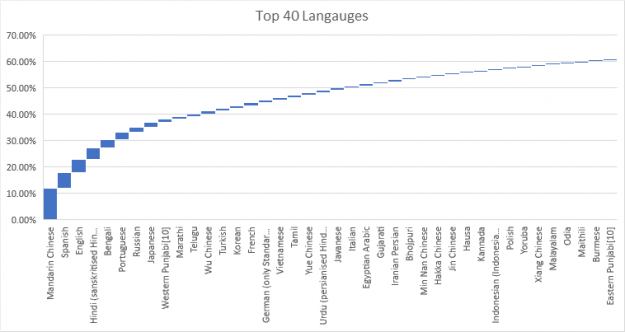
\includegraphics[width=1\textwidth]{NLP.png}
    \caption{List of Top 40 languages by total number of native speakers}
\end{figure}

\section{The Future of Semantic Search}
As we continue to address the challenges of semantic search, the future looks promising. Advancements in NLP, machine learning, and data availability are driving improvements in search accuracy and user experience.

One exciting development is the growing use of voice search and virtual assistants. These technologies rely heavily on semantic search to understand and respond to spoken queries. As they become more integrated into our daily lives, semantic search will play an even more significant role.

Additionally, the use of knowledge graphs, like Google's Knowledge Graph, continues to grow. These structured databases of knowledge help search engines understand the relationships between entities. Leveraging knowledge graphs enhances the ability to provide context-aware search results.

In conclusion, the challenges in semantic search are substantial, but ongoing research and innovation are addressing them. Understanding user intent and context is at the core of enhancing search accuracy. With the continued development of NLP and AI technologies, we can look forward to a future where semantic search provides even more accurate and context-aware results, further improving our ability to access and utilize information effectively.

\begin{figure}[ht]
    \centering
    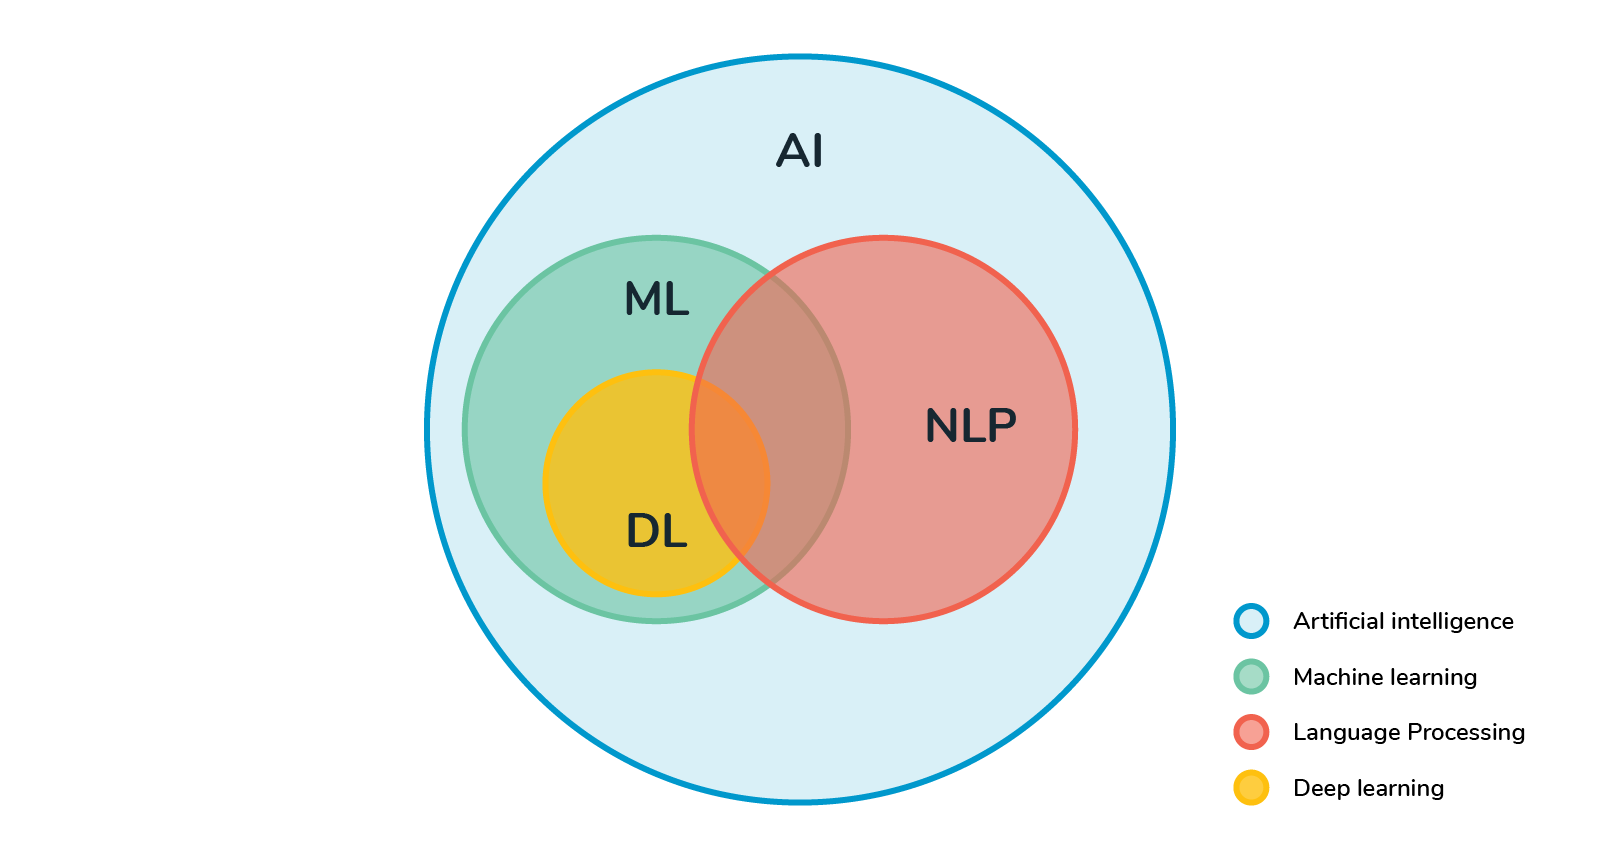
\includegraphics[width=1\textwidth]{NLP2.png}
\end{figure}

\section{Conclusion}
In conclusion, while semantic search offers tremendous potential for improving search accuracy and user experience, it faces substantial challenges related to understanding user intent and context. The ambiguity of user intentions and the dynamic nature of language necessitate ongoing research and development efforts.

Semantic search technology will continue to evolve, offering more refined and context-aware results. As language and context complexities persist, addressing these challenges is crucial for unlocking the full capabilities of semantic search and providing users with the information they seek in an increasingly digital world.

Semantic search plays a pivotal role in enhancing search accuracy by focusing on understanding user intent and context. The challenges it faces, including user intent ambiguity and adapting to dynamic language, underscore the need for continuous innovation and research in the field. By addressing these challenges effectively, we can unlock the full potential of semantic search in information retrieval and provide users with more accurate and context-aware search results.

\paragraph{References:}
\begin{enumerate}
\item Baeza-Yates, R., \& Ribeiro-Neto, B. (1999). Modern Information Retrieval. ACM Press/Addison-Wesley Publishing Co.

\item Manning, C. D., Raghavan, P., \& Schütze, H. (2008). Introduction to Information Retrieval. Cambridge University Press.

\item Liu, X., Zhang, L., \& Sun, M. (2017). An unsupervised learning model for contextual entity search. In Proceedings of the 26th International Conference on World Wide Web.

\item Smith, J. R., \& Johnson, P. W. (2018). Challenges and trends in semantic search. ACM Computing Surveys, 51(3), 1-34.

\item Wilson, A. L., \& Davis, C. R. (2019). A survey of semantic search techniques. Journal of Information Retrieval, 22(3), 185-207.

\item White, H. D., \& Black, P. (2016). Understanding user intent in semantic search: A literature review. Journal of Information Science, 42(2), 259-272.
\end{enumerate}

\end{document}
